\documentclass[twocolumn,english]{article}
\usepackage[latin9]{inputenc}
\usepackage[landscape]{geometry}
\geometry{verbose,tmargin=0.5in,bmargin=0.75in,lmargin=0.5in,rmargin=0.5in}
\setlength{\parskip}{0bp}
\setlength{\parindent}{0pt}
\usepackage{float}
\usepackage{booktabs}
\usepackage{amstext}
\usepackage{graphicx}
\usepackage{wasysym}

\makeatletter

\providecommand{\tabularnewline}{\\}




\usepackage{array}
\usepackage{multirow}
\usepackage{amsbsy}




\providecommand{\tabularnewline}{\\}

\setlength{\columnsep}{0.25in}
\usepackage{xcolor}
\usepackage{textcomp}
\usepackage{listings}
\lstset{
  tabsize=2,
  basicstyle=\small\ttfamily,
}



\usepackage{babel}
\usepackage{listings}
\renewcommand{\lstlistingname}{Listing}

\makeatother

\usepackage{babel}
\begin{document}

\title{Reference Sheet for C212 Networks and Communications}

\date{Autumn 2017}
\maketitle

\section{The Internet}

\begin{figure}[H]
\centering{}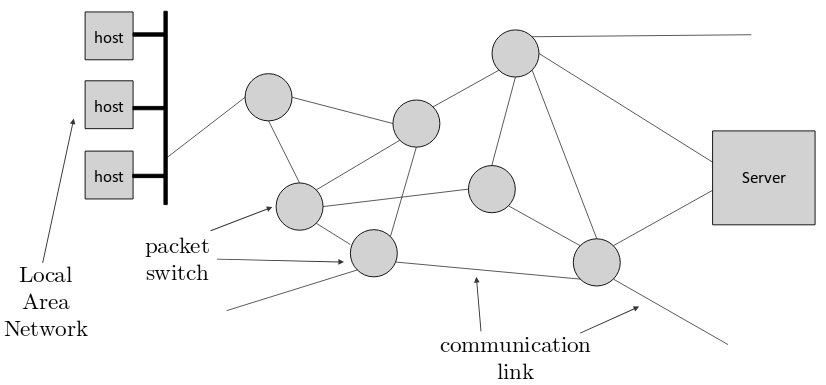
\includegraphics[width=0.75\linewidth]{img/internet}
\end{figure}

\begin{itemize}
\item \emph{Packet switch}: link-layer switch or router.
\item \emph{Communication link}: connection between packet switches and/or
end systems.
\begin{itemize}
\item Fibre optic cable, twisted pair copper wire, coaxial cable, wireless
local area links, etc.
\end{itemize}
\item \emph{Route} (\emph{path}): sequence of switches a packet goes through.
\item \emph{Protocol}: control the sending and receiving of information
between end systems/packet switches
\end{itemize}

\paragraph{Packet Switching vs Circuit Switching}

Packet-switched networks (e.g. the Internet):
\begin{enumerate}
\item Information transmitted in \emph{packets}: formatted unit of data.
\item Switches/routers operate on individual packets.
\item Switches/routers receive packets and \emph{forward} them - forwarding
decision taken on the basis of information within the packet.
\end{enumerate}
Circuit-switched networks (e.g. the telephone network):
\begin{enumerate}
\item Has a setup phase: network reserves all resources for the connection
(links, buffers, switches, etc.).
\item Links are dedicated for the entire duration of the connection.
\item Connection is destroyed and resources are freed.
\end{enumerate}
Comparing packet and circuit switching:
\begin{itemize}
\item Packet switching is \emph{connectionless}, circuit switching is \emph{connection-oriented}.
\end{itemize}
\begin{table}[H]
\centering{}%
\begin{tabular}{ccc}
\toprule 
 & \textbf{\footnotesize{}Packet Switching} & \textbf{\footnotesize{}Circuit Switching}\tabularnewline
\midrule
\emph{\footnotesize{}Setup cost} & {\footnotesize{}None} & {\footnotesize{}Expensive}\tabularnewline
\emph{\footnotesize{}Processing cost} & {\footnotesize{}For each forward} & {\footnotesize{}Little / none}\tabularnewline
\emph{\footnotesize{}Space overhead} & {\footnotesize{}For each packet} & {\footnotesize{}Little / none}\tabularnewline
\emph{\footnotesize{}Quality of Service} & {\footnotesize{}Difficult to guarantee} & {\footnotesize{}Easily guaranteed}\tabularnewline
\emph{\footnotesize{}Utilisation of links} & {\footnotesize{}Shares links - efficient} & {\footnotesize{}Limited sharing - inefficient}\tabularnewline
\bottomrule
\end{tabular}
\end{table}


\paragraph{Communication Protocols}

An agreement on how communication is to proceed.
\begin{itemize}
\item Must be an \emph{executable specification} which is \emph{unambiguous}
and \emph{complete}.
\item Needs to be able to solve \emph{addressing}, \emph{error control},
\emph{flow control}, \emph{multiplexing}/\emph{demultiplexing} and
\emph{routing}.
\end{itemize}
\begin{enumerate}
\item \emph{Handshake}: establish identities and/or contact.
\item \emph{Conversation}: exchange information.
\item \emph{Closing}: terminate conversation.
\end{enumerate}
\emph{Protocol Layering}:

\begin{figure}[H]
\centering{}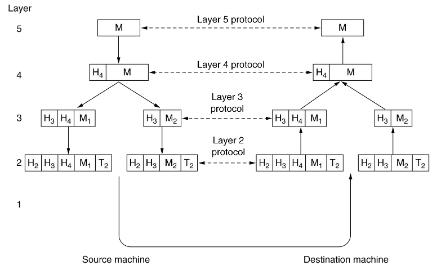
\includegraphics[width=0.5\linewidth]{img/protocol-layering}
\end{figure}

\begin{itemize}
\item \emph{Service}: set of primitives that layer provides to the layer
above.
\item \emph{Protocol}: set of rules that prescribe layout and meaning of
packets, and how the should be sent.
\item Layer $k$ puts its packet as data into a layer $k-1$ packet - which
may add a header and/or trailer.
\item \emph{Fragmentation} may be required: layer $k$ data may have to
be split accross several layer $k-1$ packets.
\end{itemize}
\emph{Internet Protocol Stack}:
\begin{enumerate}
\item \emph{Application}: defines application functionality and message
formats. E.g. Web (HTTP/HTTPS), E-mail (SMTP), BitTorrent, etc.
\item \emph{Transport}: offers connection-oriented and connectionless services.
Usually:
\begin{enumerate}
\item provides interface through \emph{sockets}, 
\item allows setting up connection, and delivering data reliably and in
the order it was sent,
\item ensures fast senders don't overwhelm slow receivers (\emph{flow control}),
\item supports \emph{secure connections}.
\end{enumerate}
\item \emph{Network (Internet)}: describes how \emph{routing} and \emph{congestion}
is solved.
\item \emph{Data Link}: allows computers to share common channel and detects
transmission errors (e.g. parity bit, checksum). E.g. Ethernet.
\item \emph{Physical}: describes transmissions of raw bits.
\end{enumerate}

\paragraph{Data Transfer}
\begin{itemize}
\item \emph{Bandwidth}: amount of information that can enter (or leave)
a connection per time unit.
\item \emph{Throughput}: actual amount of information that enters (or leaves)
connection per time unit.
\item \emph{Latency}: time it takes for one bit to go through the connection.
\item \emph{Transfer time}, $\Delta$ $=$ propagation delay (latency),
$d$ $+$ transmission delay (size, $L$ $/$ throughput, $R$).
\end{itemize}
With two hops, we also include \emph{router delay}, $d_{x}$, which
is made up of:
\begin{enumerate}
\item \emph{Processing delay}, $d_{\text{proc}}$: check bit errors, determine
output link (usually negligible).
\item \emph{Queuing delay}, $d_{q}$: time waiting at output link for transmission
(depends on average packet arrival rate, $a$):
\begin{enumerate}
\item $\frac{La}{R}\apprge$
\end{enumerate}
\end{enumerate}

\end{document}
